\chapter{模型功能及总体设计}
\label{cha:intro}

\section{模型功能}

本文提出实现的深度VO模型基于UnDeepVO\cite{li2018undeepvo},是一种使用双目摄像头数据训练,最终可以
在单目情况下运行的,具有绝对尺度的非监督深度学习方法。模型训练时只需要输入双目摄像头数
据和基本的相机内参,网络的结构和loss函数根据双目摄像头图像固有的约束和前后帧固有的空间
约束设计,无需groundtruth标定,即可得到绝对尺度的位姿变换。

\section{模型框架}

模型主要由2部分组成,第一部分为利用双目约束设计的视差生成网络。该网络利用双目图片内在的
约束,为左右目搭建压缩-解压的encoder结构,得到视差之后,即可拿到具有绝对尺度的深度图像;
第二部分需要依赖前面的视差生成网络,并且结合前后帧之间的约束,经过普通的卷积和全连接压缩
之后,分别输出一个3维translation向量和3维rotation向量,得到位姿变换。

模型的总体设计如图~\ref{fig:undeepVO_struct}


% TODO: set width
\begin{figure}
	\centering
	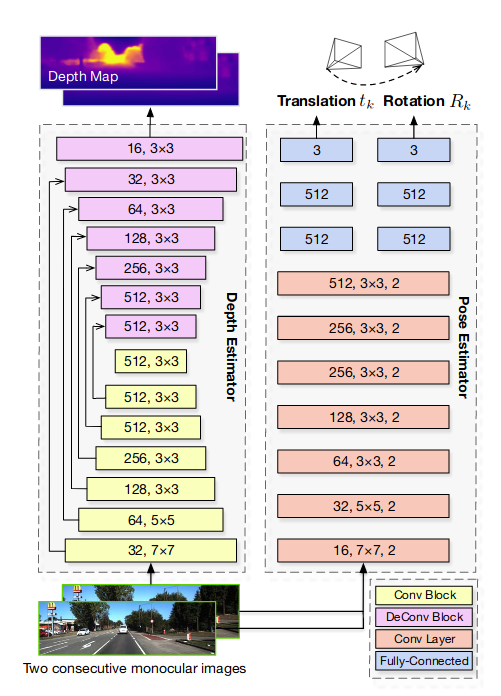
\includegraphics{undeepVO_struct.png}
	\caption{模型结构设计}
	\label{fig:undeepVO_struct}
\end{figure}

本文是项目的阶段性报告,为保证实验的正确性,促使实验顺利进行,笔者在第一阶段着重实现了基于
非监督学习的视差生成网络,即模型的第一部分。原因有二:视差生成网络有一定的独立性,可以在没
有位姿生成网络的情况下单独训练和验证;并且,视差生成网络是整个网络的基石,第二部分位姿生
成网络的成功直接的依赖第一部分的结果。因此,在下文的报告中,笔者会着重介绍视差生成网络的
设计,原理与部分实验结果,对于模型第二部分仅做简单的介绍。

\subsection{视差网络的模型设计}

视差是双目方法中常用的一种工具,它是基于单孔相机和双目相机模型的,对同一位点在左右目不同的
位置差的一种表示,由于太过基础,对于视差的具体表示和处理方式本文暂时掠过不提,仅对模型的设计
和表示作出说明。

在训练过程中,视差生成网络的输入是2张等大的3通道RGB图片(即左右目图片),我们为图片的每一个
像素点计算视差,即输出也是2张与输入尺寸相同的图片,但是是单通道的(视差当然是一个数)。那么,
根据这个特性,其实我们很容易想到,模型应该有一个显示的压缩-解压过程,对左右目的信息进行特征
提取。

根据图~\ref{fig:undeepVO_struct}可以看到,视差生成网络的确是典型的encoder--decoder
模型,在特征提取阶段我们使用$strip > 1$的卷积方式不断对图片进行压缩,得到特征之后再使用
反卷积将信息升样到我们希望的格式。

在实际的编码过程中,模型的压缩和解压其实有很多种选择,目前流行的最典型的encoder-decoder
网络且适合当前任务的主要有两种,一种是VGG\cite{simonyan2014very}网络,一种是
ResNet\cite{he2016deep},笔者经过慎重的考量在第一阶段
的实验中使用了VGG网络,因为一方面VGG网络比ResNet网络简单一些,另一方面由于VGG发布时间较
早,笔者对它也更为熟悉。

在具体实现时,encoder和decoder分别7层,每层使用stride=1及stride=2的卷积进行压缩,激活函数
使用elu,采用的通道数和kernel size分别为(32, 7), (64, 5), (128, 3), (256, 3),
(512, 3), (512, 3), (512, 3)。

\subsection{位姿生成网络的模型设计}

同视差生成网络相比,位姿估计网络的设计就要简单的多。因为这个网络的输出是2个三维向量,而输入
则是连续的双目图像,因此对于这个部分来说,信息的流动是一个单项压缩的过程,由图~\ref{fig:undeepVO_struct}
也可以看出。

在设计过程中,只需要不断的使用卷积对图片进行压缩,最后使用全连接层将数据整合到我们想要的形式
即可。当然,对这个网络来说,科学的loss设计是及其重要的,也决定着网络是否成功,对于loss的具体
设计和公式表达,我们将在下一章节进行讨论。



